\section{Bitcoin}

Non è propriamente una moneta, è un sistema di pagamento.
Sfrutta protocolli crittografici sia per generare nuova moneta che per attestare il possesso della valuta da parte degli utenti.

Nasce nel 2008 con la pubblicazione di \emph{Bitcoin: a peer to peer Electronic cash system} a cura di \emph{Satoshi Nakamoto} (pseudonimo per una persona o un gruppo ancora ignoto).
Nel 2009 viene rilasciato il primo software per partecipare (bitcoin-core) ed il 3 Gennaio 2009 viene creato il \emph{blocco genesi}.

Questo sistema è costituito da un libro contabile (\emph{ledger}) pubblico e distribuito costituito da singoli blocchi concatenati tra di loro: la \emph{blockchain}.
Con il primo blocco si sono creati i primi 50 bitcoin.
Ogni volta che si riesce ad aggiungere un nuovo blocco si creano nuovi bitcoin ed ogni 4 anni circa si dimezza la moneta generata (inizialmente 50 bitcoin per blocco, ora 6.25 per blocco).
La generazione ha un tempo massimo infatti nel 2140 l'aggiunta di blocchi non genererà più nuova moneta.

Il 12 Gennaio 2009 avviene la prima transazione: Satoshi Nakamoto invia 10 Bitcoin ad Hal Finney (il creatore del proof of work).

Nel 2010 avviene la prima transazione commerciale, vengono pagate due pizze.

\subsection{Come funziona?}
Dopo aver scaricato il software necessario l'utente genera una sua coppia di chiavi pubblica e privata:
\begin{itemize}
    \item $K_A[pub]$: costituisce l'indirizzo identificativo dell'utente, si usa per ricevere Bitcoin e per verificare la firma
    \item $K_A[priv]$: si usa per firmare le transazioni e quindi spendere
\end{itemize}

\subsubsection{Wallet}
E' l' insieme delle credenziali che attestano la proprietà in BTC di un utente: la coppia indirizzo/chiave privata in quanto ogni utente ne possiede una assieme al software di gestione

\subsubsection{Transazione}
E' lo scambio di valuta tra due utenti. Immaginiamo che A voglia inviare $x$ BTC a B: il messaggio avrà la forma:
$$ m = address_A - x - address_B$$
verrà corredato da un hash:
$$ h = SHA-256(m)$$
e dalla firma:
$$ f = D(h, K_A[priv]) $$
la coppia $<m, f>$ verrà quindi diffusa nella rete peer-to-peer in broadcast.

Essendo su un sistema distribuito il destinatario deve aspettare che la rete convalidi la transazione e richiede almeno 10 minuti.
Dopo 10 minuti il blocco verrà aggiunto alla blockchain, bisogna poi aspettare l'aggiunta di altri 6 blocchi al nostro ramo per essere sicuri al 100\% di aver compiuto una transazione.

All'interno di una transazione i bitcoin non possono essere frazionati:
\begin{table}[ht!]
    \centering
    \begin{tabular}{c c c}
         &  & 0.5 Bitcoin ad Alice \\
        Bob riceve 50 Bitcoin &  $\xrightarrow{transazione A}$ &\\
         & & 49.5 Bitcoin a Bob
    \end{tabular}
\end{table}

Successivamente Alice può spendere o meno i bitcoin ricevuti.
Può anche mettere assieme più indirizzi di input:
\begin{table}[ht!]
    \centering
    \begin{tabular}{c c c}
        Alice riceve 0.5 Bitcoin & & \\
        Alice riceve 0.1 Bitcoin & $\xrightarrow{transazione B}$ & utente riceve 0.8 Bitcoin\\
        Alice riceve 0.2 Bitcoin & &
    \end{tabular}
\end{table}

Si possono spendere solo output non spesi di precedenti transazioni che avevano noi come destinatario.
La somma degli input deve sempre essere maggiore o uguale alla somma degli output, se è uguale pagamenti normali, se è maggiore quelli in più vengono aggiunti al primo che convalida il blocco (perché può aggiungere questo movimento).
Per incentivare questa conferma si usa quindi lasciare questa \emph{fee} al miner.

\subsubsection{Validazione}
Gli utenti ricevono dal broadcast queste transazioni, le controllano (cercano nel passato se la valuta è presente nel conto di chi invia) le mettono assieme a gruppi (100, 200 anche 1000) e poi provano ad aggiungerle alla blockchain.
Ci sono vari modi per aggiungerli, noi vedremo il \emph{proof of work}.

Tutto questo è fatto per evitare che sia possibile il double spending: creare più transazioni quasi contemporaneamente, questo potrebbe succedere nel periodo in cui avviene la validazione, ma si risolve con questa divisione in blocchi.

\subsection{Com'è fatto un blocco}

\begin{figure}[H]
    \centering
    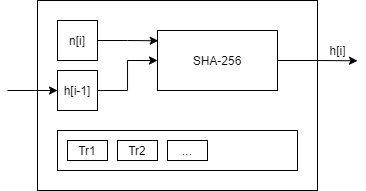
\includegraphics[width=300px]{Bitcoin_1.png}
\end{figure}

Prendo un tot di transazioni, le raggruppo, aggiungo la transazione finale che mi dirige la ricompensa, costruisco la porzione $Tr_{i}$.

Nel blocco c'è $h_{i-1}$ cioè l'hash del blocco precedente. Nel blocco c'è $n_i$ detto \emph{nonce}, un intero.

Di queste informazioni faccio l'hash SHA-256 ed ottengo $h_i$. La richiesta è quella di ottenere un $h_i < $ di una certa soglia fissata dal sistema.
Ciò che si fa è quindi iterare su tutti i nonce e cercare un hash con $T$ zeri all'inizio.
Il parametro $T$ è fissato dal sistema e varia in base alla potenza della rete.
Questo è scelto in modo da portare il tempo di validazione di un blocco a circa 10 minuti.
In media ci vogliono $2^T$ tentativi.

Chi cerca di attaccare un nuovo blocco è detto \emph{miner} e sono i nodi che validano le transazioni.

Si parla di \emph{validazione tramite mining}.

Cercare il nonce è difficile, verificarlo invece è semplice quindi chi trova il nonce lo diffonde in broadcast a tutti i nodi, gli altri lo verificano, controllano la validità delle transazioni ed esprimono il loro consenso: prendono il nuovo nodo e cercheranno di attaccare nuovi nodi ad esso.

Se la rete ad un certo punto ha delle biforcazioni si tende a privilegiare i rami con più transazioni perché è più probabile che siano accettati da tutta la rete.

La proof of work è quindi questa ricerca del nonce.

\subsection{Mining pool}
Inizialmente Bitcoin doveva essere democratico e quindi tutti avrebbero potuto partecipare al mining, quello che è successo invece è stato che alcuni piccoli gruppi di utenti hanno unito le forze e messo a disposizione grande hardware per minare tutti assieme, ci si spartisce quindi lo spazio di ricerca del nonce e si dividono i profitti tra i vari partecipanti.

\subsection{Aspetti sociali}
Il mining ormai è poco sociale in quanto lo fanno in pochi e guadagnagno in pochi.
Inoltre si perde un sacco di energia elettrica per calcoli "inutili".
Sono state quindi sviluppate altre monete digitali che dirigono il proof work verso ambiti di ricerca per non rendere tutta questa energia elettrica sprecata

\subsection{Attacchi alla blockchain}
Per attaccare la blockchain si deve disporre di una grande potenza di calcolo.
Si possono mettere d'accordo più persone per far si che si attacchino blocchi a piacere.
Si deve disporre del 51\% della rete che è abbastanza difficile, se avessi questa potenza però sarebbe più remunerativo giocare onestamente.












